%Over the course of this report we have refered to, and approximated, the distribution of variouss classifications of prime numbers. Using now our implementation of Helfgott's origianl code we seek to present the legitimacy of said distributions and also reflect on the quality of the code which we have written. The specific distributions to be presented are those of the regular prime numbers, the twin primes, and a the frequency of various prime gaps will also be presented. For each of these implementations have slight modifications been made to the code, which will be briefly discussed.

Genom rapportens gång har vi hänvisat till, och uppskattat fördelningen av, ett antal klasser av primtal och deras egenskaper. 
Nu kommer vi att redovisa några resultat som ovan nämnda Python-program givit.
Vi börjar med att räkna primtal i ett intervall och jämföra det med primtalssatsen, detta i syftet att övertyga oss om kodens legitimitet. 
Sedan undersöker vi den möjliga sanningen av en hypotetisk fördelning för primtalstvillingar. 
Slutligen redovisas frekvensen av primtalsgap, och mönster som uppträder däri.

\subsubsection{Fördelningen av primtal}\label{app.primes.title}
%Beginning with the classic example of the set of prime numbers, below is illustrated the distribution predicted by the familiar x over log x from sieve theory/Chebychev, the more accurate lorgarithmic integral Li(x), and the actual number of primes found in using our implementation. In order to generate the following graph, no new sieving methods were introduced, simply the counting fucntion in Appendix X

Vi börjar med att jämföra antalet primtal hittat med \textsc{NewSegSiev} emot fördelningen som ges av primtalssatsen, nämligen
\begin{equation}
    \pi(x) \sim \text{Li}(x) = \int_2^x\frac{1}{\log t}dt\label{app.primes.PNT}.
\end{equation}
För att skapa följande figur använder vi vår implementering av Helfgotts kod och en enkel räknefunktion.

\begin{figure}[H]
    \centering
    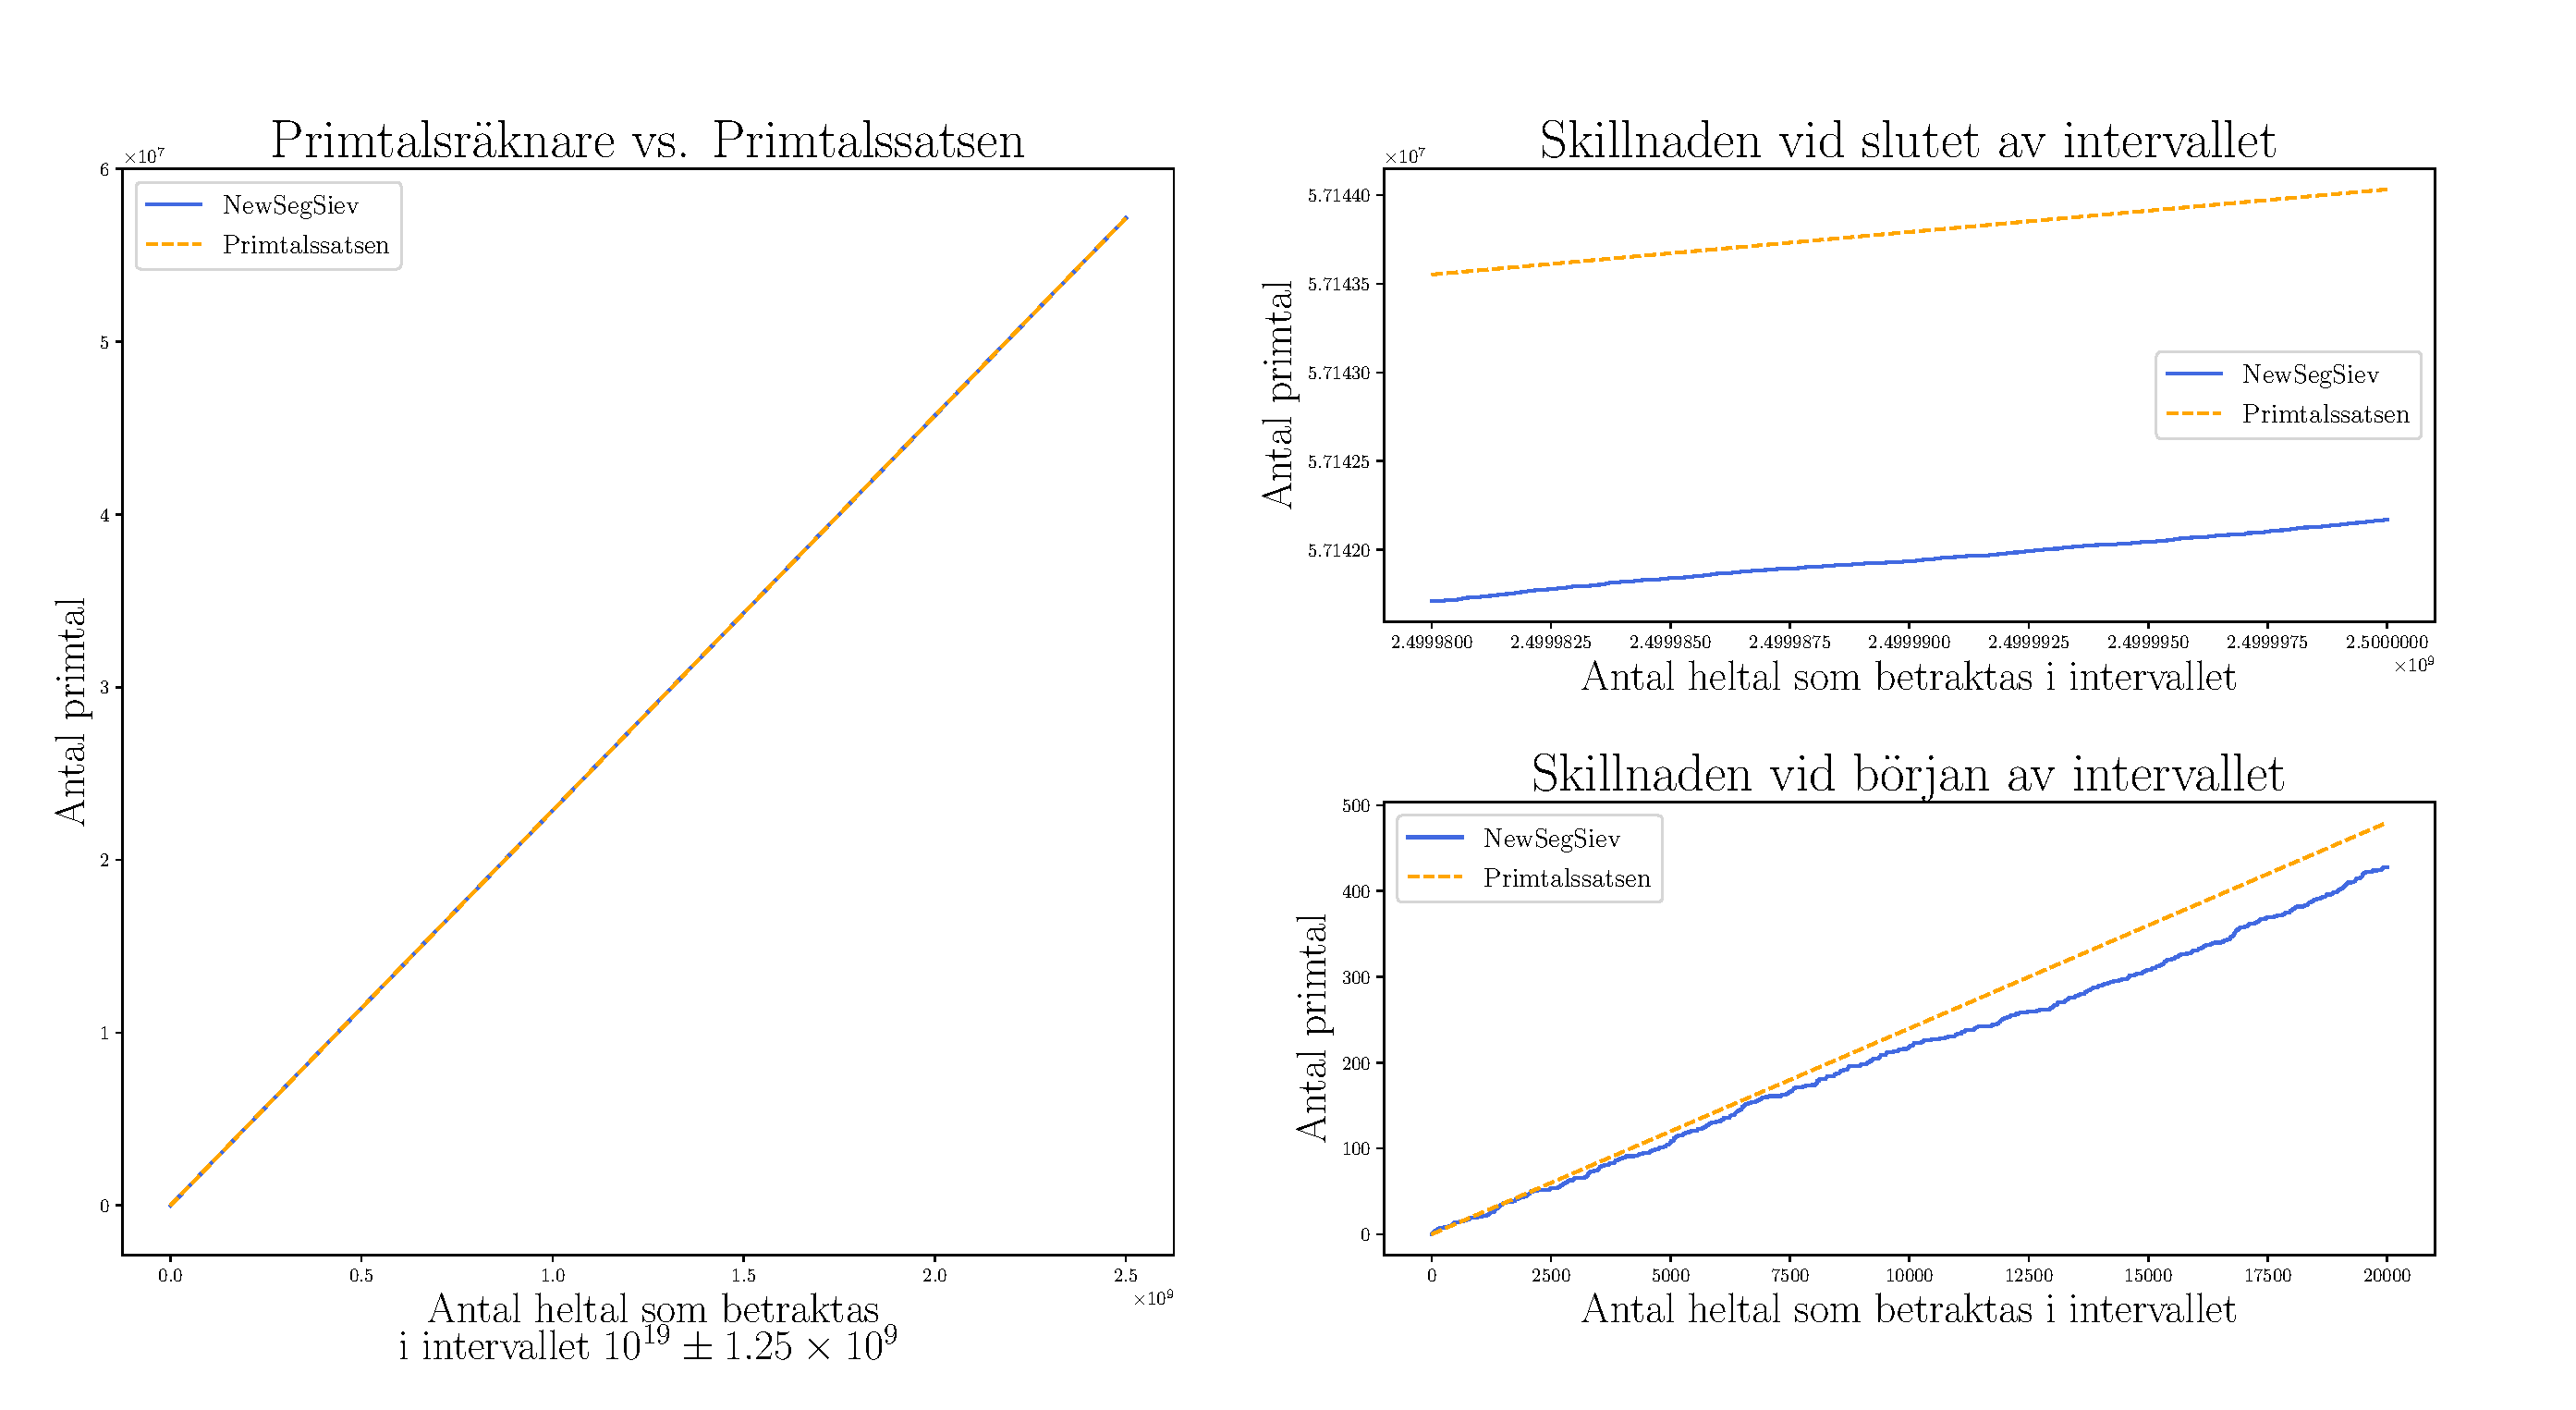
\includegraphics[width = \textwidth]{coen/Images/Primes.pdf}
    \caption{I figuren till vänster redovisas antalet primtal som förväntas enligt primtalssatsen, \textit{orange}, och antalet primtal som hittades enligt \textsc{NewSegSiev}, \textit{blå}, då \(n = 10^{19}\), \(\Delta = 1.25\cdot10^{9}\), och \(K = 2.5\). 
    Notera gärna att kurvorna ligger nästan på varandra. 
    I grafen till höger redovisas inzoomade versioner av grafen till vänster för att visa skillnaden mellan vår uppskattning och det som förväntas vid början av intervallet, där algoritmen returnerar kring 100 färre primtal än förväntat, och vid slutet av intervallet, där algoritmen returnerar kring 2000 färre.
    Dock att kurvorna inte ligger på varandra kan förvantas till en viss grad eftersom det finns ett fel i \ref{app.primes.PNT} vilket inte visas.}
    %This graph shows the relative distributions of primees as per the aforementioned fucntions. Notice that while x over log x appears relatively close for smaller x the logarithmic integral approximation is a near exact match for the true distribution, so much so that the code line is hidden.
    \label{fig:res.prime}
\end{figure}
%As shown in figure X, should we believe in the PNT it seems as though our code does indeed find the correct number of primes. The rather large error in the x over log x estimate is indicative/reflective of one of the limitations highlighted in Section XXX, namely the impact of the error terms and their reconcillation with the main terms. Howeve, there doest exist a deeper link between the x over log x estimate and that of the logarithmic integral. Throguh the use of integral wizardry you can decompose the logarithmic integral into a series of terms, the first of which being x over log x with the remainder being of the order of sqrt(x). This then accounts for the increase in error as x grows. Thiese kinds of approximations for the prime counting function can also be rather naturally extrapolated to those for twin primes, as discussed below.

Som vi ser i vänstra grafen av figur \ref{fig:res.prime}, då vi nu tror på primtalssatsen så verkar det som vår kod hittar det korrekta antalet primtal i intervallet, eftersom skillnaden mellan kurvorna är nästa osynlig på makronivå. 
Att de inte ligger exakt på varandra är huvudsakligen beroende på felet vilket inte visas i \eqref{app.primes.PNT}.
Notera att vi normaliserar felet vid början av intervallet eftersom betraktar skillnaden \(\text{Li}(x) - \text{Li}(n - \Delta)\), \(x\in[n-\Delta,\; n+\Delta]\) då vi plottar antalet förvantat primtal i intervallet.
Att vår kod hittar ungefär 100 färre primtal än förväntat efter 20 000 heltal och ungefär 2000 färre primtal efter \(2.5\times10^9\) heltal är mycket rimligt då vi anser att felet i \eqref{app.primes.PNT} kan bäst vara \(O(2\Delta)^{1/2 + \varepsilon}),\; \varepsilon > 0\), under antagandet att Riemannhypotesen stämmer \cite[Kapitel 5]{RiemannErr}.

Vi väljer \textit{n} till \(10^{19}\) för att först och främst undersöka så långt ifrån noll som möjligt, med tanke på att försöka öka skillnaden mellan antalet primtal som genererades och antalet primtal som förväntades i intervallet\footnote{Att \textit{n} inte valdes större i detta fallet är på grund av körningstiden för koden.}.
Att vi väljer \(\Delta\) till \(1.25\times10^9\) för att använda Helfgotts förbättringar i \textsc{NewSegSiev}, \textsc{DiophAppr} funktionen, och för att göra det krävs en specifik storlek på intervallet.
Slutligen väljer vi \textit{K} till 2.5 för att det är minsta \textit{K}:et som kan väljas enligt Helfgott.
Tillsammans bildar dessa parametrar, med stöd från primtalssatsen, en bra bas för de följande tillämpning då vi sparar bitarray:n och läser in den istället för att generar alla primtal inför varje körning.

\subsubsection{Fördelningen av primtalstvillingar}
%Continuing our presentation of various sets of prime's distributions, next we turn to the other recurring theme of twin primes. The following figure illustrates the distributions of twin primes as predicted by x over log squared x and the second order logarithmic integral against those primes found using our implementation. It should be noted that a rather simple help function, Appendix XXX, was written which searches for non twin primes in the prime list and removes them.

Med hjälp av de primtal vi hittade i \ref{app.primes.title}, vänder vi oss nu till primtalstvillingar. Det finns ingen sats för primtalstvillingar motsvarande primtalssatsen, dock så finns det en förmodan framlagd av Hardy och Littlewood \cite[Förmodan B]{Hardy} som lyder
\begin{equation}
    \pi_2(x) \sim 2\text{C}_2\cdot \text{Li}_2(x) = 2\text{C}_2\int_2^x\frac{1}{(\log t)^2}dt\label{app.twins.TWN}
\end{equation}
där \(\text{C}_2 = 0.66016...\) är primtalstvillingskonstanten \cite{TwinPrimeConstant}. Jämför vi den hypotetiska fördelningen emot antalet primtalstvillingar vi har genererat, så får vi följande figur.

\begin{figure}[H]
    \centering
    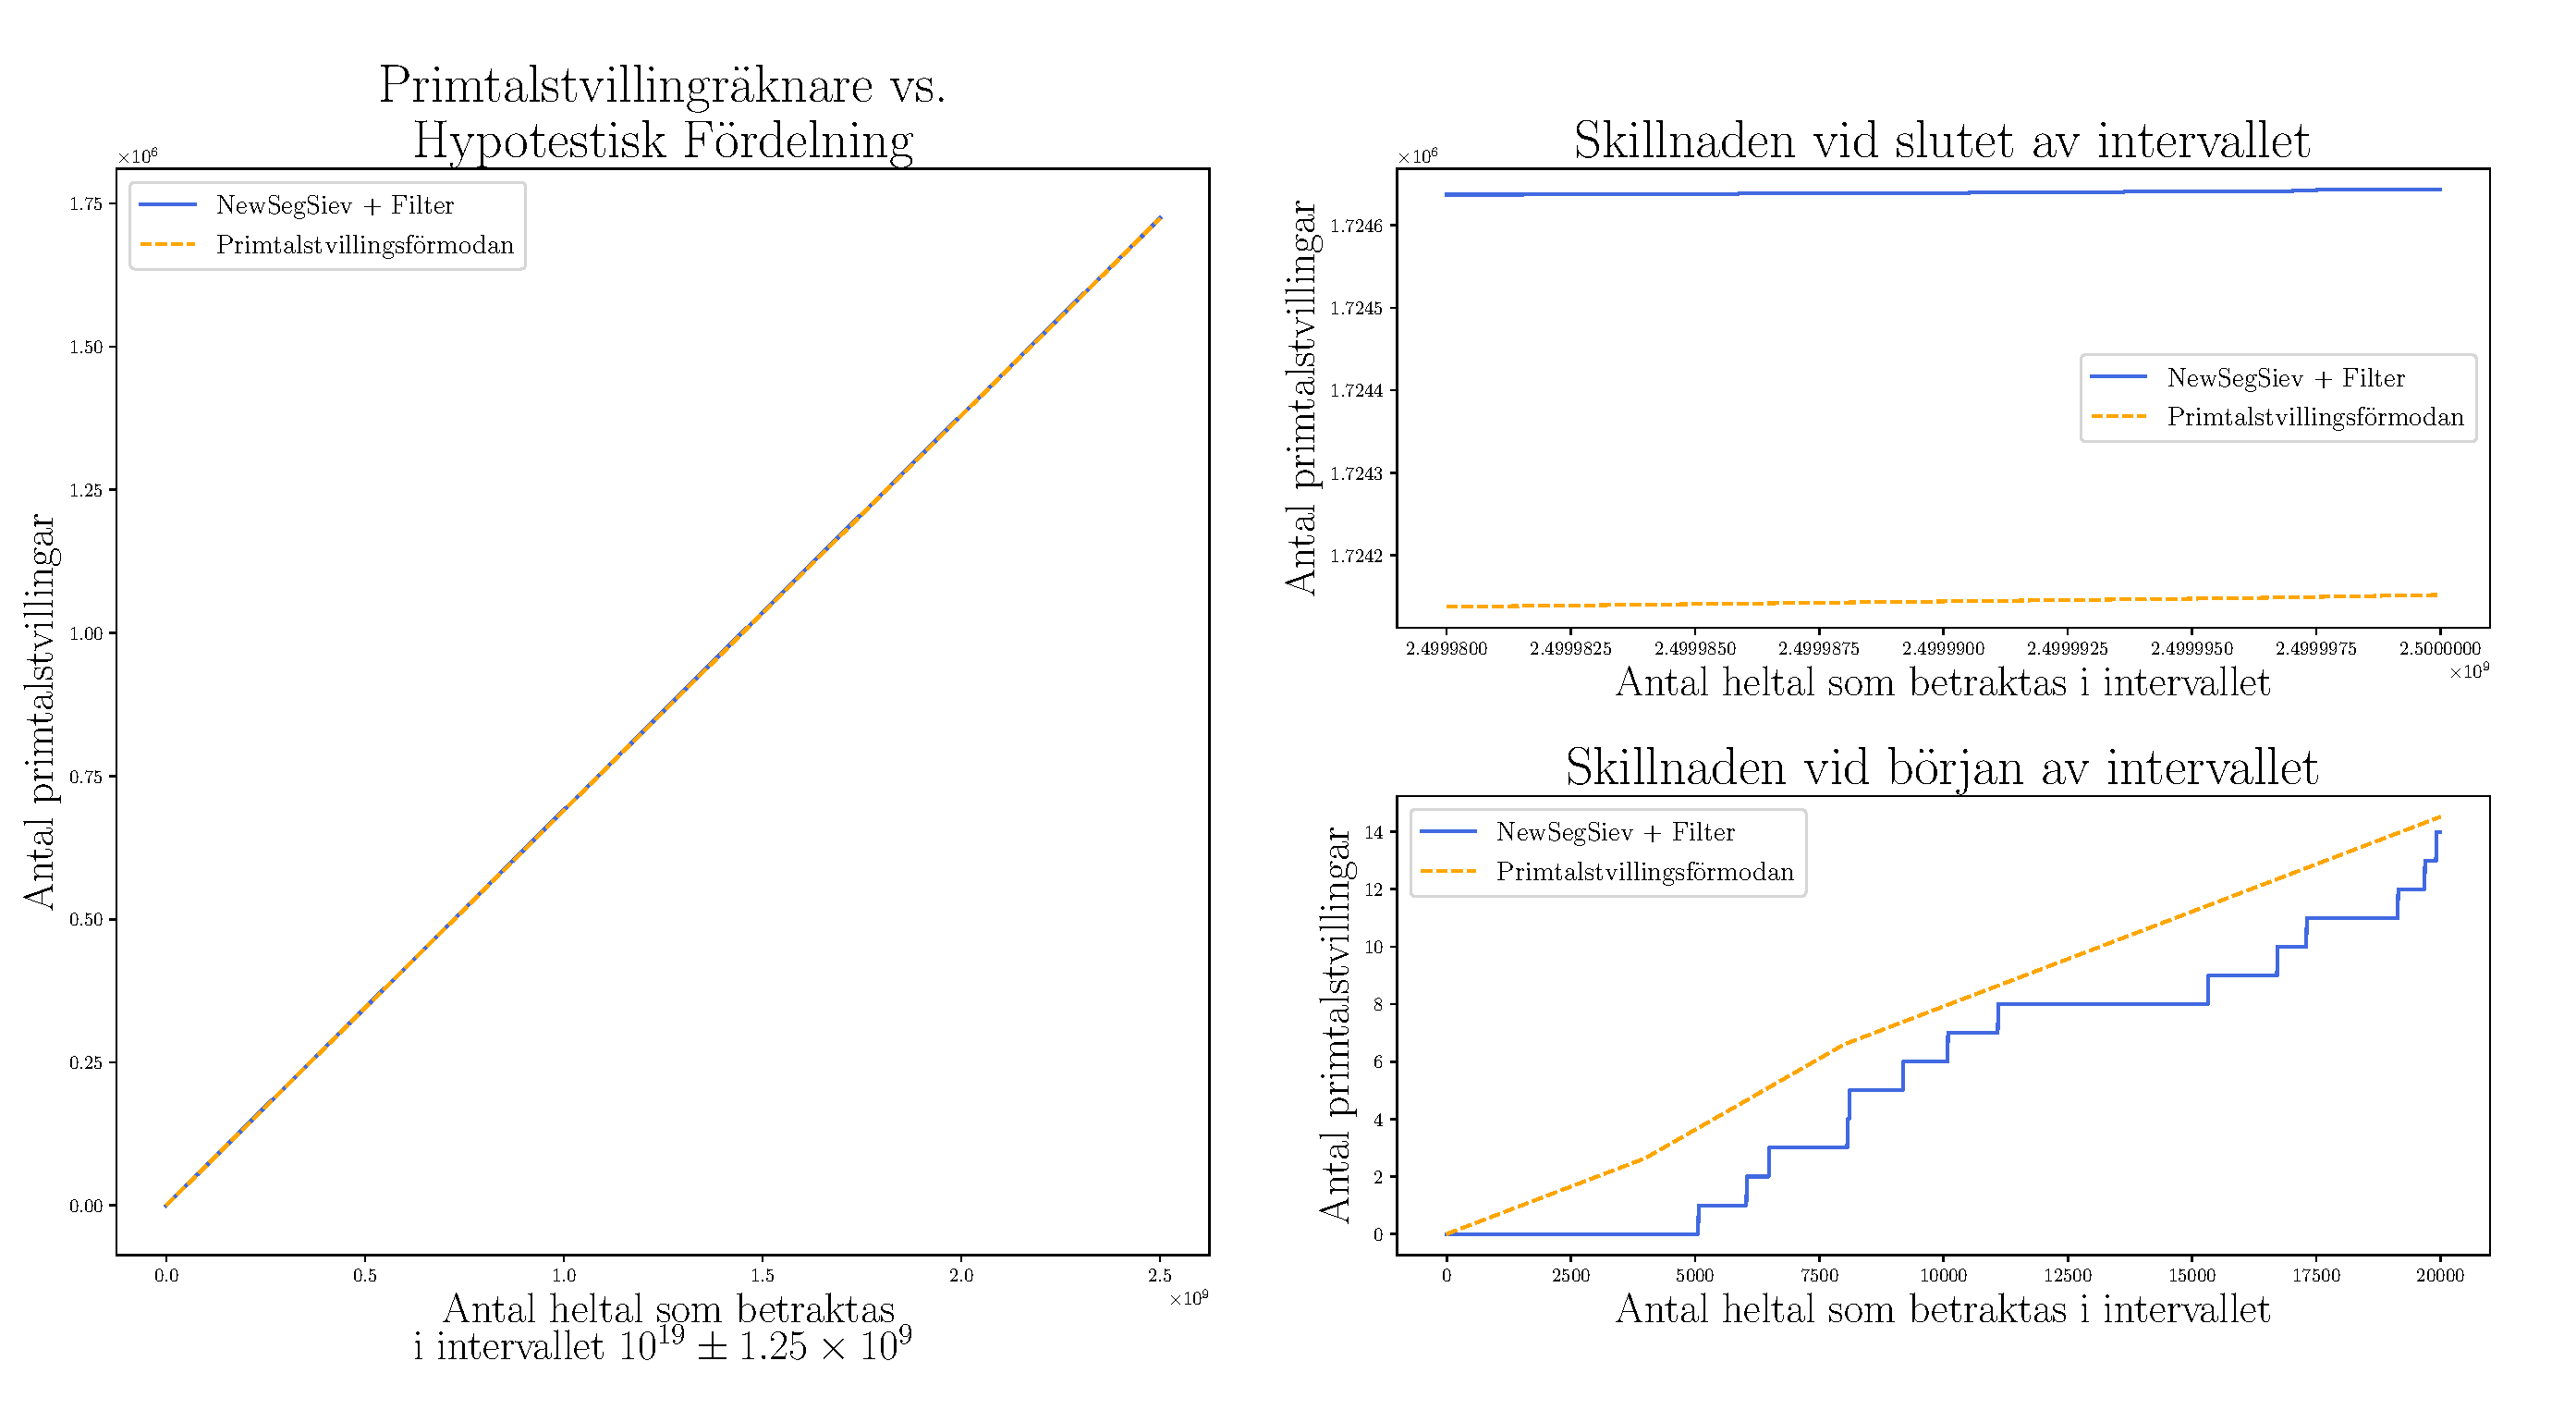
\includegraphics[width = \textwidth]{coen/Images/TwinPrimesNoKapp.pdf}
    \caption{I grafen till vänster redovisas antalet primtalstvillingar som förväntas enligt den hypotetiska fördelningen, \textit{orange}, och de primtalstvillingar som hittades enligt \textsc{NewSegSiev}, \textit{blå}, då \(n = 10^{19}\), \(\Delta = 1.25\times10^9\), och \(\text{C}_2\) har avrundats till 0.66. Notera återigen att kurvorna ligger nästan på varandra. I graferna till höger så redovisas inzoomade versioner av grafen till vänster. 
    Översta grafen till höger visar skillnaden mellan antalet primtalstvilling vi har hittat och antalet som förväntas vid slutet av intervallet, där algoritmen returnerar 500 fler primtalstvillingar. Efter de första 20 000 heltalen i intervallet så har algoritmen genererat nästan det exakta antalet primtalstvillingar som förväntas.}
    %This graph shows the relative distributions of the twin primes as per the aforementioned fucntions. Notice once again the accuarcy of the logarithmic integral, once again hiding our code line, as opposed to that of C x over log squared x, where the constant is 2*C_2, or 2 times the twin prime constant (discussed below).
    \label{fig:res.twins}
\end{figure}

Datan i figur \ref{fig:res.twins} ger oss några intressanta insikter angående primtalstvillingar. 
Den första är att datan ger stöd till den hypotetiska fördelningen av primtalstvillingar. 
Som vi ser i grafen till vänster, då vi nu litar på koden så kan den hypotetiska fördelningen av primtalstvillingar definitivt vara rimligt eftersom kurvorna verkar ligga på varandra.
Vid början av intervallet är skillnaden mellan det förväntade antalet primtalstvillingar och antalet som hittades maximalt 4, och vid slutet så har skillnaden ökat till ungefär 500.
I sammanhanget av ett intervall av längd \(2.5\times10^9\) så är en skillnad av 500 ekvivalent med en avvikelse av \(2\times 10^{-7}\) mer primtalstvillingar per heltal än vad som förväntades.
Att antalet primtalstvillingar blir större än det hypotetiskt förväntade antalet vid slutet på intervallet beror möjligen på att vi avrundar \(\text{C}_2\) till 0.66 i kombination med att vi normaliserar felet vid början av intervallet precis som i föregående tillämpning.
Dock så kunde avrundningen av \(\text{C}_2\) tillsammans med normaliseringen av felet också ha ökat antalet förväntade primtalstvillingar till mer än vad det skulle egentligen vara. 
I sin tur leder detta till att förmodan verkar stödjas av vår implementering mer än vad den borde vara.

Den andra insikten grafen ger är kopplad till anmärkningen vid slutet på tillämpningen av Eratosthenes såll i avsnitt \ref{Eratosthenes}.
Vi noterar där att Bruns sats medför att andelen primtalstvillingar av primtalen är relativt liten och då vi jämför graferna i figurer \ref{fig:res.prime} och \ref{fig:res.twins} kan vi se den förväntade relationen.
Vi ser direkt att antalet primtal bland de första 20 000 heltal i den första figuren är kring 400 vilket är ungefär 30 gånger fler än antalet primtalstvillingar som finns i de första 20000 heltal som betraktas.
När vi istället tittar vid slutet av intervallet blir kvoten mellan antalet primtal och antalet primtalstvillingar inte mindre; den ökar något till ungefär en faktor av 33 fler enkla primtal jämfört med tvillingar.

Vi kan inte använda vår kod som bevis för den hypotetiska fördelningen för primtalstvillingar. 
Dock så ger den oss en känsla för om fördelningen verkar rimlig i detta fallet, vilket den gör. Vi kan också få en känsla för hur få primtalstvillingar det finns jämfört mot antalet primtal, vilket underlättar förståelsen för en av sållteorins första stora framsteg, nämligen Bruns sats.


%There are a number of things to discuss regardng the above figure. 
\subsubsection{Frekvens av primtalsgap}

Vi fortsätter med att ge visualiseringar av egenskaper av de primtal vi har genererat genom att undersöka frekvensen av olika storlekar av primtalsgap. 
En primtalsgap är avståndet mellan ett primtal och sitt efterföljande primtal.
Man kan, med hjälp av primtalssatsen, visa att det förväntade avståndet mellan ett primtal \(p_n\) och nästa, \(p_{n+1}\), är \(\log p_n\).
För att ge intuition för det förväntade avståndet och mer stöd till vår kod så analyserar vi nu de primtalsgap som finns i listan av primtal vi generad. Datan redovisas i nästa figur.

\begin{figure}
    \centering
    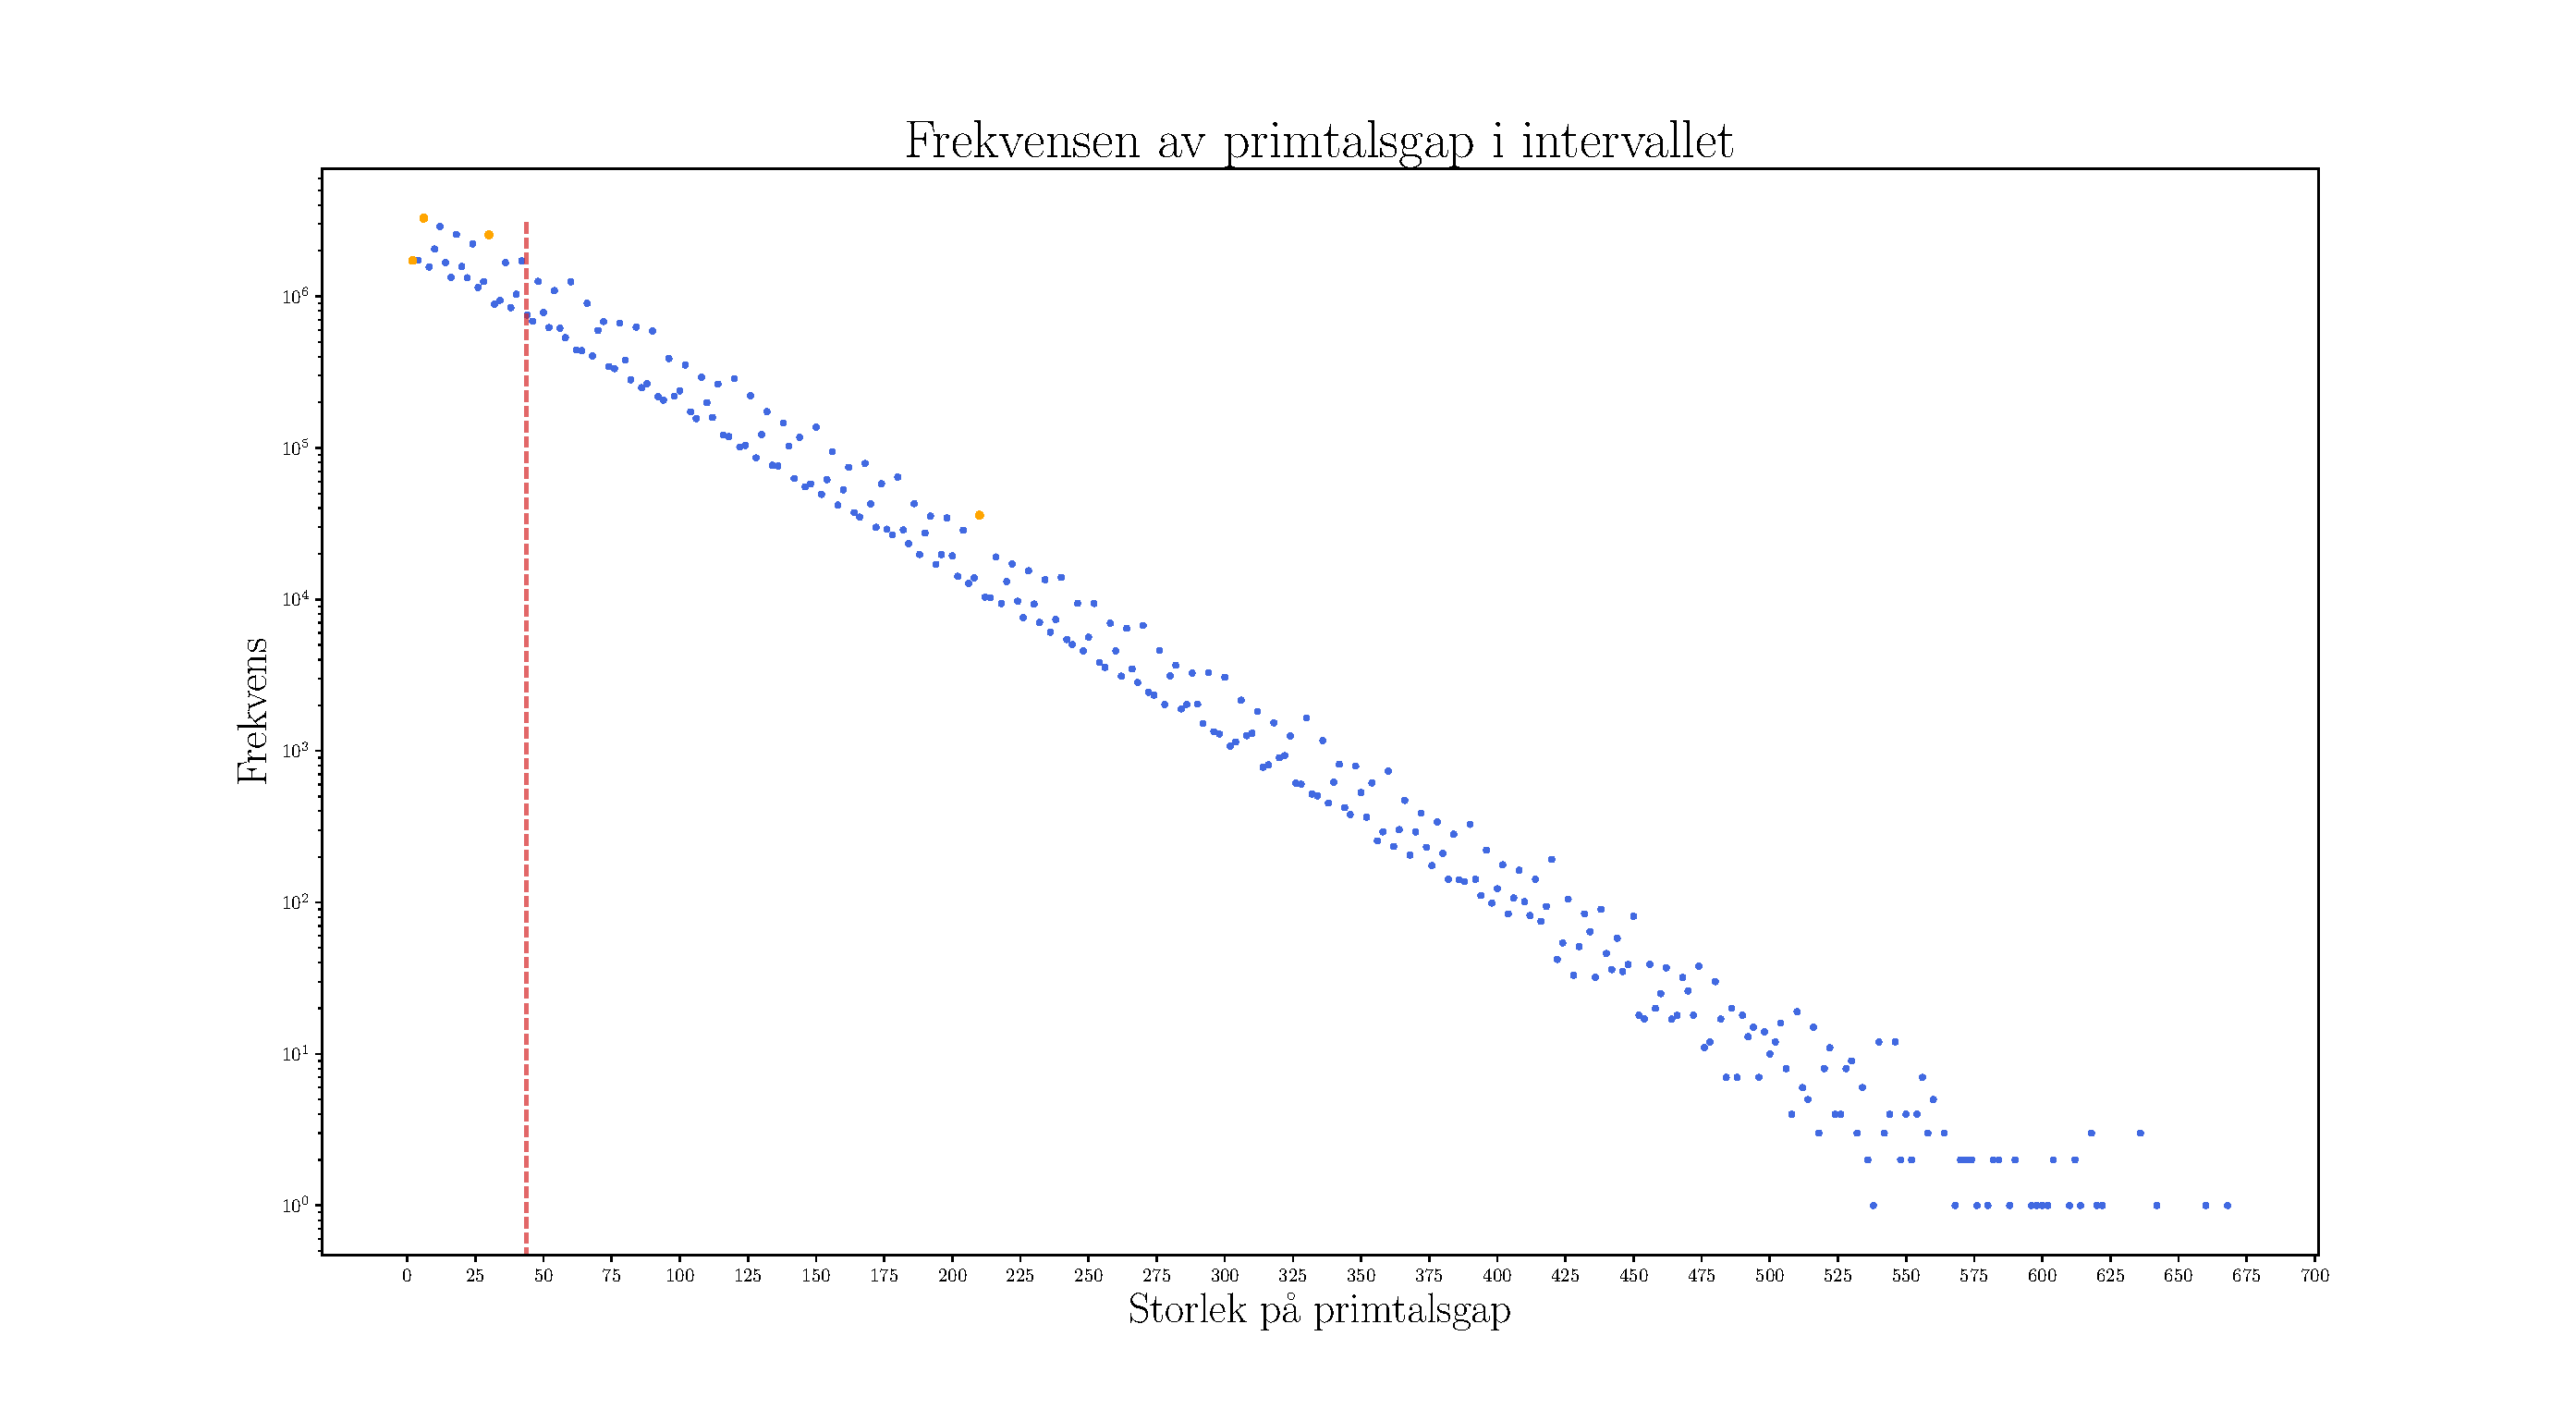
\includegraphics[width = \textwidth]{coen/Images/GapsNoKapps.pdf}
    \caption{I figuren så redovisas frekvensen på olika stora primtalsgap i det intervallet som undersöktes tidigare, då \(n = 10^{19}\), \(\Delta = 1.25\cdot10^{9}\), och \(K = 2.5\). Notera att y-axeln är logaritmerad på grund av hur hög frekvensen är för små primtalsgaper. 
    Dem orange prickarna anger frekvensen på primtalsgap vars storlek är en primorial (en produkt av de första \textit{n} primtalen).
    Röda linjen markerar den genomsnittliga storleken på primtalsgap i vårt intervall vilket är 43.705.}
    \label{fig:res.gap}
\end{figure}

I figur \ref{fig:res.gap} får vi några insikter kring beteendet av primtalsgap i vårt intervall. 
Den mest överraskande aspekten av grafen, för någon som har inte sett en sådan graf förut, är hur rak den är då vi logaritmerar y-axeln.
Detta påpekar att frekvensen på primtalsgap minskar exponentiellt då dess längd ökar. 
Vi ser att det vanligaste storlek på primtalsgap i vårt intervall var 6 och längsta avståndet mellan två primtal var av längd 668.
En till detalj vilken inte kan läsas lätt av figuren är att det finns par av primtal i intervallet där avståndet mellan dem är lika med varje jämn tal upp till och inklusive 560.
Vi nämnde tidigare att den förväntade storleken på primtalsgapet för ett primtal \textit{p} tills nästa primtal är \(\log(p)\). 
Då vi uppskattar storleksordningen på våra primtal med \(10^{19}\) får vi att den förväntade storleken på ett primtalsgap i intervallet är ungefär 43.7491.
Vi ser att många primtalsgap överstiger detta och ännu fler är mycket mindre, dock då vi beräknar den genomsnittliga storkleken på primtalsgap i vårt intervall så får vi det till 43.7505.
Återigen stödjer detta resultat legitimiteten av vår kod eftersom vår kod reflekterar vad som har bevisats i primtalssatsen.

Om vi återgår till primtalstvillingar så säger figuren även något om dem. 
Vi kan se att om alla primtal med ett visst primtalsgap till nästa primtal skulle betraktas vara lika speciellt som primtalstvillingar, då skulle primtalstvillingar vara de sjunde vanligaste typ av primtal i vårt intervall, och består av 3 procent av alla primtal i intervallet.

Till sist, figur \ref{fig:res.gap} ger intuition för en sats som antyddes till kortfattat i inledningden. 
Satsen säger att det finns oändligt många par av primtal med maximalt 600 steg emellan sig. 
Detta betyder att, även för de stora primtalen måste det finnas primtal relativt nära varandra.
I vårt intervall har vi att nästan alla primtal som genererades var inom 600 steg från varandra trots att vi arbetar med så stort tal.
Detta bevisades med hjälp av nya sållmetoder, specifikt Goldston-Pintz-Yıldırım metoder utvecklades år 2005 \cite{GPY}.
I Maynards artikel så liknar vikterna som använts i beviset de som används i Selbergs såll, fast på en ännu mer allmän form. 
I nuläget så har 600 steg reducerades ned till 246. 
Ett mål med att fortsätta minska längden är att en dag reducera det till 2 och därmed bevisa primtalstviliingshypotesen.

Såsom mycket annat angående primtal, finns det åtminstone en förmodan kopplad till dessa frekvenser ovan och vilket primtalsgap är mest frekvent upp till en given övregräns. 
Som vi ser i figur \ref{fig:res.gap} är 6, den andra orange pricken, den mest frekventa storleken på primtalsgap i vårt intervall, och det som är speciellt med 6 är att det är produkten av de första två primtalen. 
Vi ser också från figuren att 30, den tredje orange pricken, vilket är produkten av de första 3 primtalen, hoppar upp lite från översta delen av bandet, och även 210, den fjärde orange pricken, med. Förmodan är då att varje \textit{primorial}, produkten av de första \textit{m} primtalen, någon gång blir "hoppmästaren".
Förmodan har undersökts direkt med hjälp av numeriska uppskattningsmetoder \cite{primeGap} som har lyckats visa att 6 är hoppmästaren fram till \(\approx 1.74\cdot10^{35}\) och att 30 är hoppmästaren mellan föregående och \(\approx 10^{425}\).

%Nutidens forskningen kring primtalsgap representerar kulmen på sållteorins teoretisk tillämpning.
%Teorin har utvecklats markant under de senaste hundra åren och tillämpats framgångsrikt på många problem inom talteori.
%Om teorins utveckling fortsätter på denna bana, så kommer fler och fler problem kunna lösas med hjälp av bättre och bättre sållteori.
